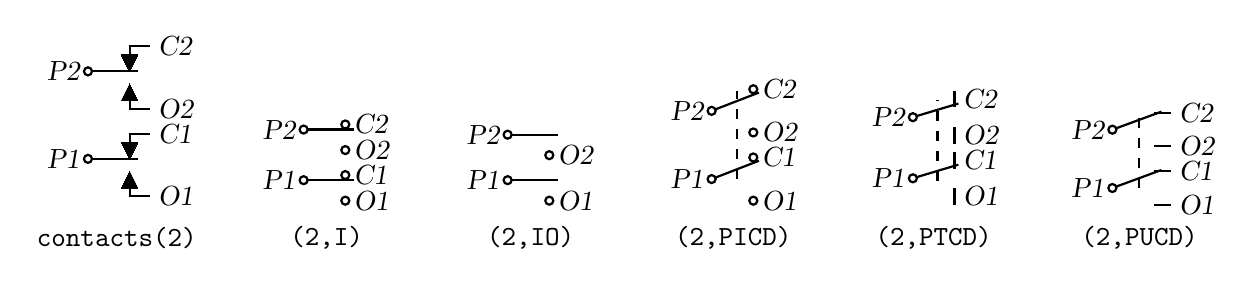
\begin{tikzpicture}[scale=2.54]
% dpic version 2020.03.01 option -g for TikZ and PGF 1.01
\ifx\dpiclw\undefined\newdimen\dpiclw\fi
\global\def\dpicdraw{\draw[line width=\dpiclw]}
\global\def\dpicstop{;}
\dpiclw=0.8bp
\dpiclw=0.8bp
\dpicdraw[fill=white](0.02,-0.1875) circle (0.007874in)\dpicstop
\dpicdraw (0.04,-0.1875)
 --(0.27,-0.1875)\dpicstop
\filldraw[line width=0bp](0.186667,-0.104167)
 --(0.228333,-0.1875)
 --(0.27,-0.104167) --cycle\dpicstop
\dpicdraw (0.228333,-0.175077)
 --(0.228333,-0.0625)
 --(0.328333,-0.0625)\dpicstop
\filldraw[line width=0bp](0.27,-0.333333)
 --(0.228333,-0.25)
 --(0.186667,-0.333333) --cycle\dpicstop
\dpicdraw (0.228333,-0.262423)
 --(0.228333,-0.375)
 --(0.328333,-0.375)\dpicstop
\dpicdraw[fill=white](0.02,0.25) circle (0.007874in)\dpicstop
\dpicdraw (0.04,0.25)
 --(0.27,0.25)\dpicstop
\filldraw[line width=0bp](0.186667,0.333333)
 --(0.228333,0.25)
 --(0.27,0.333333) --cycle\dpicstop
\dpicdraw (0.228333,0.262423)
 --(0.228333,0.375)
 --(0.328333,0.375)\dpicstop
\filldraw[line width=0bp](0.27,0.104167)
 --(0.228333,0.1875)
 --(0.186667,0.104167) --cycle\dpicstop
\dpicdraw (0.228333,0.175077)
 --(0.228333,0.0625)
 --(0.328333,0.0625)\dpicstop
\draw (0.164167,-0.583333) node{\tt contacts(2)};
\draw (0,-0.1875) node[left=-2bp]{\sl P1};
\draw (0.348333,-0.375) node[right=-2bp]{\sl O1};
\draw (0.348333,-0.0625) node[right=-2bp]{\sl C1};
\draw (0,0.25) node[left=-2bp]{\sl P2};
\draw (0.348333,0.0625) node[right=-2bp]{\sl O2};
\draw (0.348333,0.375) node[right=-2bp]{\sl C2};
\dpicdraw[fill=white](1.098333,-0.294167) circle (0.007874in)\dpicstop
\dpicdraw (1.118333,-0.294167)
 --(1.348333,-0.294167)\dpicstop
\dpicdraw[fill=white](1.306667,-0.268611) circle (0.007874in)\dpicstop
\dpicdraw[fill=white](1.306667,-0.396667) circle (0.007874in)\dpicstop
\dpicdraw[fill=white](1.098333,-0.041111) circle (0.007874in)\dpicstop
\dpicdraw (1.118333,-0.041111)
 --(1.348333,-0.041111)\dpicstop
\dpicdraw[fill=white](1.306667,-0.015556) circle (0.007874in)\dpicstop
\dpicdraw[fill=white](1.306667,-0.143611) circle (0.007874in)\dpicstop
\draw (1.213333,-0.583333) node{\tt (2,I)};
\draw (1.078333,-0.294167) node[left=-2bp]{\sl P1};
\draw (1.326667,-0.396667) node[right=-2bp]{\sl O1};
\draw (1.326667,-0.268611) node[right=-2bp]{\sl C1};
\draw (1.078333,-0.041111) node[left=-2bp]{\sl P2};
\draw (1.326667,-0.143611) node[right=-2bp]{\sl O2};
\draw (1.326667,-0.015556) node[right=-2bp]{\sl C2};
\dpicdraw[fill=white](2.118333,-0.294167) circle (0.007874in)\dpicstop
\dpicdraw (2.138333,-0.294167)
 --(2.368333,-0.294167)\dpicstop
\dpicdraw[fill=white](2.326667,-0.396667) circle (0.007874in)\dpicstop
\dpicdraw[fill=white](2.118333,-0.066667) circle (0.007874in)\dpicstop
\dpicdraw (2.138333,-0.066667)
 --(2.368333,-0.066667)\dpicstop
\dpicdraw[fill=white](2.326667,-0.169167) circle (0.007874in)\dpicstop
\draw (2.233333,-0.583333) node{\tt (2,IO)};
\draw (2.098333,-0.294167) node[left=-2bp]{\sl P1};
\draw (2.346667,-0.396667) node[right=-2bp]{\sl O1};
\draw (2.098333,-0.066667) node[left=-2bp]{\sl P2};
\draw (2.346667,-0.169167) node[right=-2bp]{\sl O2};
\dpicdraw[fill=white](3.138333,-0.288611) circle (0.007874in)\dpicstop
\dpicdraw[fill=white](3.346667,-0.180556) circle (0.007874in)\dpicstop
\dpicdraw[fill=white](3.346667,-0.396667) circle (0.007874in)\dpicstop
\dpicdraw (3.156984,-0.281391)
 --(3.374544,-0.197167)\dpicstop
\dpicdraw[fill=white](3.138333,0.0525) circle (0.007874in)\dpicstop
\dpicdraw[fill=white](3.346667,0.160556) circle (0.007874in)\dpicstop
\dpicdraw[fill=white](3.346667,-0.055556) circle (0.007874in)\dpicstop
\dpicdraw (3.156984,0.05972)
 --(3.374544,0.143944)\dpicstop
\dpicdraw[dash pattern=on 0.05in off 0.05in](3.265764,-0.289279)
 --(3.265764,0.151832)\dpicstop
\draw (3.246439,-0.583333) node{\tt (2,PICD)};
\draw (3.118333,-0.288611) node[left=-2bp]{\sl P1};
\draw (3.366667,-0.396667) node[right=-2bp]{\sl O1};
\draw (3.366667,-0.180556) node[right=-2bp]{\sl C1};
\draw (3.118333,0.0525) node[left=-2bp]{\sl P2};
\draw (3.366667,-0.055556) node[right=-2bp]{\sl O2};
\draw (3.366667,0.160556) node[right=-2bp]{\sl C2};
\dpicdraw[fill=white](4.144544,-0.284722) circle (0.007874in)\dpicstop
\dpicdraw (4.352877,-0.236111)
 --(4.352877,-0.152778)\dpicstop
\dpicdraw (4.352877,-0.416667)
 --(4.352877,-0.333333)\dpicstop
\dpicdraw (4.1637,-0.278975)
 --(4.372034,-0.216475)\dpicstop
\dpicdraw[fill=white](4.144544,0.020833) circle (0.007874in)\dpicstop
\dpicdraw (4.352877,0.069444)
 --(4.352877,0.152778)\dpicstop
\dpicdraw (4.352877,-0.111111)
 --(4.352877,-0.027778)\dpicstop
\dpicdraw (4.1637,0.02658)
 --(4.372034,0.08908)\dpicstop
\dpicdraw[dash pattern=on 0.05in off 0.05in](4.267867,-0.297725)
 --(4.267867,0.10783)\dpicstop
\draw (4.248289,-0.583333) node{\tt (2,PTCD)};
\draw (4.124544,-0.284722) node[left=-2bp]{\sl P1};
\draw (4.372877,-0.375) node[right=-2bp]{\sl O1};
\draw (4.372877,-0.194444) node[right=-2bp]{\sl C1};
\draw (4.124544,0.020833) node[left=-2bp]{\sl P2};
\draw (4.372877,-0.069444) node[right=-2bp]{\sl O2};
\draw (4.372877,0.111111) node[right=-2bp]{\sl C2};
\dpicdraw[fill=white](5.142034,-0.333333) circle (0.007874in)\dpicstop
\dpicdraw (5.4337,-0.25)
 --(5.350367,-0.25)\dpicstop
\dpicdraw (5.4337,-0.416667)
 --(5.350367,-0.416667)\dpicstop
\dpicdraw (5.160807,-0.326437)
 --(5.387659,-0.243104)\dpicstop
\dpicdraw[fill=white](5.142034,-0.041667) circle (0.007874in)\dpicstop
\dpicdraw (5.4337,0.041667)
 --(5.350367,0.041667)\dpicstop
\dpicdraw (5.4337,-0.125)
 --(5.350367,-0.125)\dpicstop
\dpicdraw (5.160807,-0.03477)
 --(5.387659,0.048563)\dpicstop
\dpicdraw[dash pattern=on 0.05in off 0.05in](5.274233,-0.33477)
 --(5.274233,0.056896)\dpicstop
\draw (5.277867,-0.583333) node{\tt (2,PUCD)};
\draw (5.122034,-0.333333) node[left=-2bp]{\sl P1};
\draw (5.4537,-0.416667) node[right=-2bp]{\sl O1};
\draw (5.4537,-0.25) node[right=-2bp]{\sl C1};
\draw (5.122034,-0.041667) node[left=-2bp]{\sl P2};
\draw (5.4537,-0.125) node[right=-2bp]{\sl O2};
\draw (5.4537,0.041667) node[right=-2bp]{\sl C2};
\end{tikzpicture}
\vspace*{-0.5\baselineskip}
